\chapter*{Proposition 27}

\begin{figure*}[ht]
    \begin{center}
    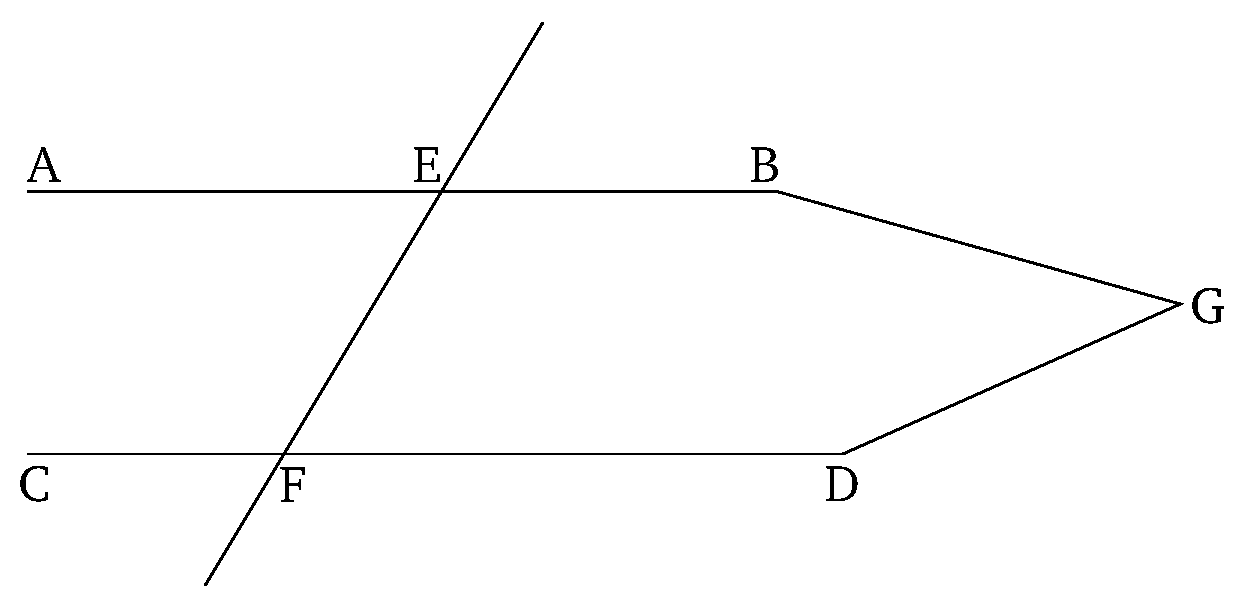
\includegraphics[width=0.5\linewidth]{figures/fig27e.eps}
    \label{fig:prop_27}
    \end{center}
\end{figure*}

If a straight-line falling across two straight-lines makes  the alternate
angles equal to one another then the (two) straight-lines will be parallel to
one another.

For let the straight-line $EF$, falling across the two straight-lines $AB$ and
$CD$, make the alternate angles $AEF$ and $EFD$ equal to one another.
I say that $AB$ and $CD$ are parallel.

For if not, being produced, $AB$ and $CD$ will certainly meet together:
either in the direction of $B$ and $D$, or (in the
direction) of $A$ and $C$ [Def.~\ref{def:23}]. Let them have been
produced, and let them meet together in the direction of $B$ and $D$ at
 (point) $G$. So, for the triangle $GEF$, the external angle
$AEF$ is equal to the interior and opposite (angle) $EFG$. The
very thing is impossible [Prop.~1.16]. Thus, being produced, $AB$ and $CD$
will not meet together in the direction of $B$ and $D$. Similarly, 
it can be shown that neither (will they meet together) in (the
direction of) $A$ and $C$. But  (straight-lines) meeting in neither
direction are parallel [Def.~\ref{def:23}]. Thus, $AB$ and $CD$ are parallel.

Thus, if a straight-line falling across two straight-lines makes  the alternate
angles equal to one another then the (two) straight-lines will be parallel (to
one another). (Which is) the very thing it was required to show.


\section*{Commentary}

\begin{proposition}\label{proposition_27}\lean{Elements.Book1.proposition_27}\leanok
    $A$ and $E$ are two distcint points on the line $AE$. $F$ and $D$ are two distinct points on $FD$. $E$ and $F$ are two distinct points on $EF$. $A$ and $D$ are on different sides of $EF$. $\angle~AEF = \angle~EFD$. Then, $AE$ and $FD$ must be parallel.
\end{proposition}
\begin{proof}
    \uses{proposition_16}\leanok
    See the original proof by Euclid.
\end{proof}

